\section{How can we Slow down Aging?}

\subsection{Overview}

\begin{frame}[c]{Goal of Anti-Aging Research}
    \large
    As I understand it, the goal of anti-aging research is \textbf{the extension of the human lifespan}.

    Ideally by stopping aging or achieving neglegible senescence.
    Intermediate goals include slowing down aging, and increasing QUALYs (QUality-Adjusted-Life-Years).
    \pnote{
        neglegible senescence = not aging biologically \\
        \par
        neglegible senescence is further out, we are \\
        barely able to slow it down a few percent \\
        \par
        aim for longevity escape velocity
    }
\end{frame}

\begin{frame}[c]{Potential Strategies to Slow down Aging}
    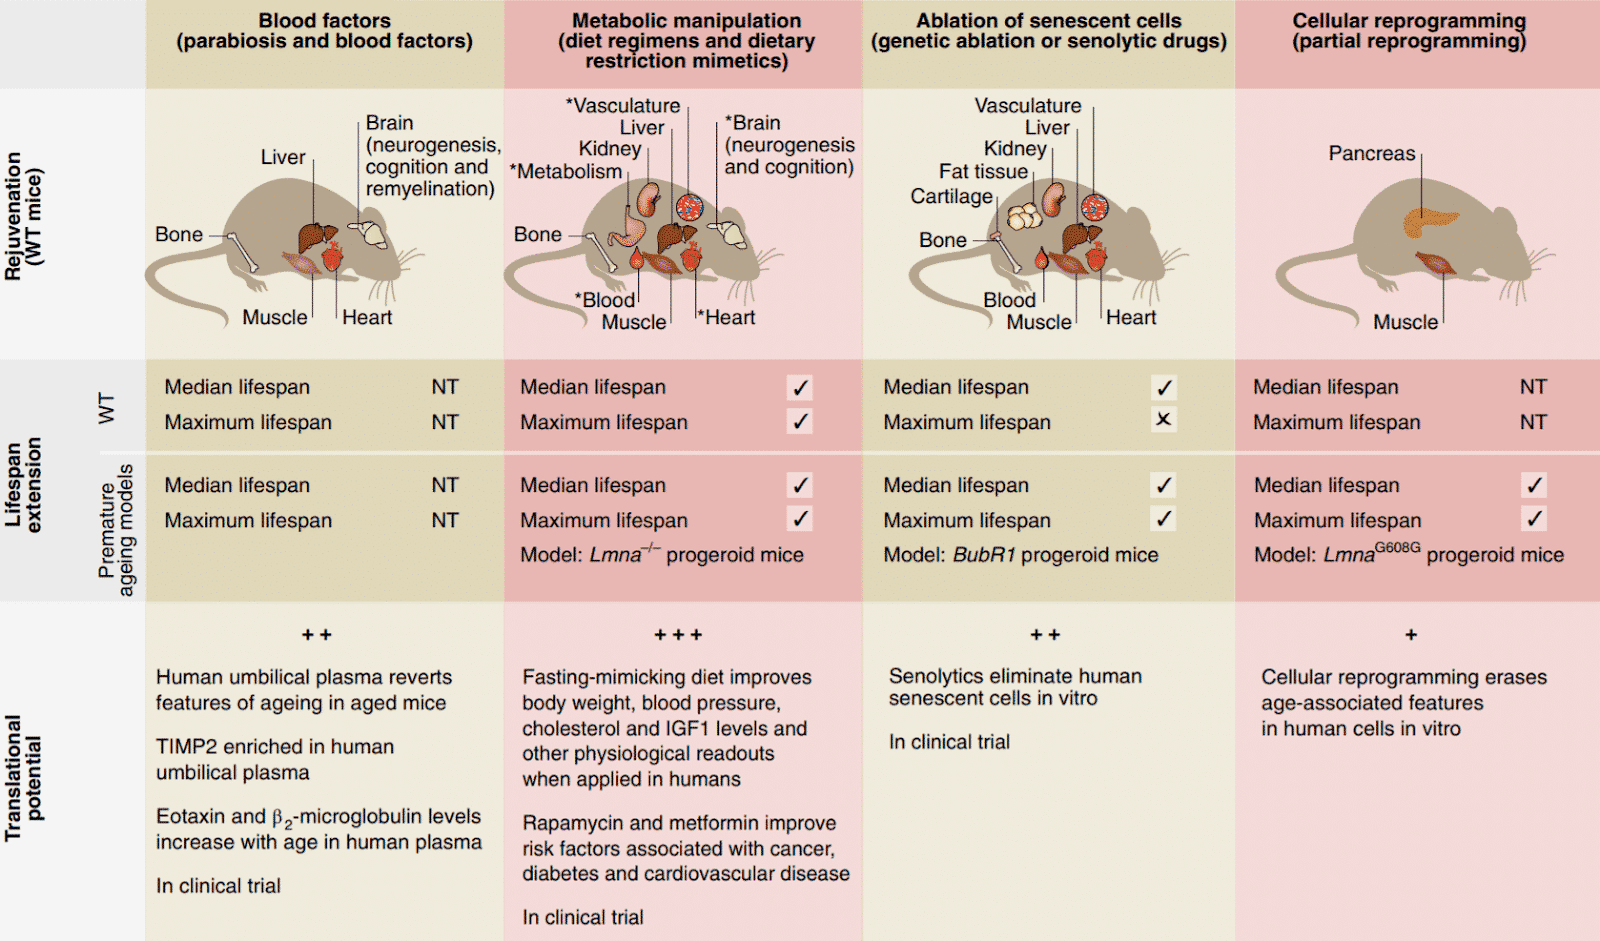
\includegraphics[width=\textwidth]{strategy_comparison_short} \\
    Source: \cite{mahmoudi2019turning}, picture modified

    \pnote{
        Comparison of rejuvenation strategies \\
        Currently highest potential, but more exist
        \par
        We will take a deeper look at all of them \\
        No need to study overview for long
        \par
        Treatment initiated midlife or later \\
        \par
        Next: Parabiosis
    }

    % \pnote{A comparison of the four emerging rejuvenation strategies: blood factors,
    % metabolic manipulation, ablation of senescent cells and cellular
    % reprogramming. The figure depicts the features that improve when treatment
    % in mice is initiated at midlife or later. The top panel shows organs or
    % tissues that exhibit a rejuvenated phenotype in wild-type (WT) mice. For
    % rapamycin, features that have been shown to improve also in young mice
    % following treatment are indicated with an asterisk (*). The effect on
    % lifespan, proposed primary mode (or modes) of action and possible
    % trade-offs of these strategies are also presented. Finally, the
    % translational potential in humans is indicated by the increasing number of
    % plus signs (+) based on present evidence in human ageing and current
    % feasibility. NT, not tested. Question marks indicate possible modes of
    % action and trade-offs.}
\end{frame}


\subsection{Parabiosis}

\begin{frame}[c]{Parabiosis (Blood Exchange)}
    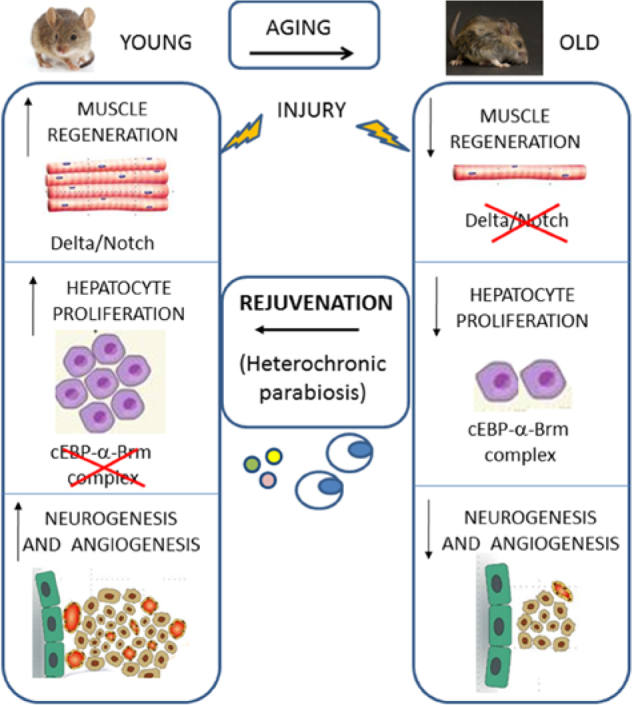
\includegraphics[height=0.85\textheight]{parabiosis_effects} \\
    Source: \cite{conese2017fountain}
    \pnote{
        Connecting blood circulation of old and young \\
        Benefits to old, donwsides to young mice \\
        Can be brought to biological equilibrium
        \par
        Works by Hormones, Immune defenses and \\
        other Growth Factors/regulation in the blood \\
        as well as nutrients and stem cells
        \par
        hepatocyte = important liver cell \\
        angiogenesis = forming new blood vessels
        \par
        Next: How good is it? (Evaluation)
    }
\end{frame}

\begin{frame}[c]{Method Evaluation: Parabiosis}
    \large
    % Parabiosis (heterochronic parabiosis) is putting young blood into old mice, to make the old mice biologically younger. This is achieved in the lab by connecting the circulatory systems of young mice and old mice. Certain factors in the blood help to rejuvenate muscle, heart brain and liver tissues in old mice and restore their biological function.

% Equivalent procedures that modify the compounds within blood in humans such as apheresis (blood filtering) could be used to slow aging in humans and thereby prevent or slow the progression of many types of age-related diseases including Alzheimer's disease.

% Recently, a group of Russian biohackers recently took part in the first plasma dilution experiments in humans. In a research context, the safety and effectiveness of apheresis is being tested in a clinical trial in humans by the company Alkahest.

    \textbf{Hallmarks affected}:
    \begin{aquote}{\cite{conese2017fountain}}
        In principle, the heterochonic parabiosis reverts all phenotypic and molecular hallmarks of ageing by transferring soluble factors and cells.
    \end{aquote}
    % \begin{itemize}[<+(1)->]
    %     \item Stem cell exhaustion
    %     \item Cellular senescence
    %     \item Altered intercellular communication
    % \end{itemize}
    % parabiosis reverses age-related decline by targeting several hallmarks of aging including stem cell exhaustion, cellular senescence and altered intercellular communication (inflammation).

    \pause
    Alternatives: Blood Filtering and (Growth) Hormone Therapy. \\
    \pause
    \textbf{Status: In clinical trial}, e.g. \cite{AStudyto73:online}.
    \pnote{
        soluble = 'Löslich' \\
        also transfers bone marrow (stem cells) \\
        Source: \cite{lukic2005shared} \\
        \par
        Alternatives, because downsides for young \\
        mice not neglegible
    }
\end{frame}


\subsection{Metabolic Manipulation}

\begin{frame}[c]{Dietary Restriction in D. melanogaster (Fruit Fly)}
    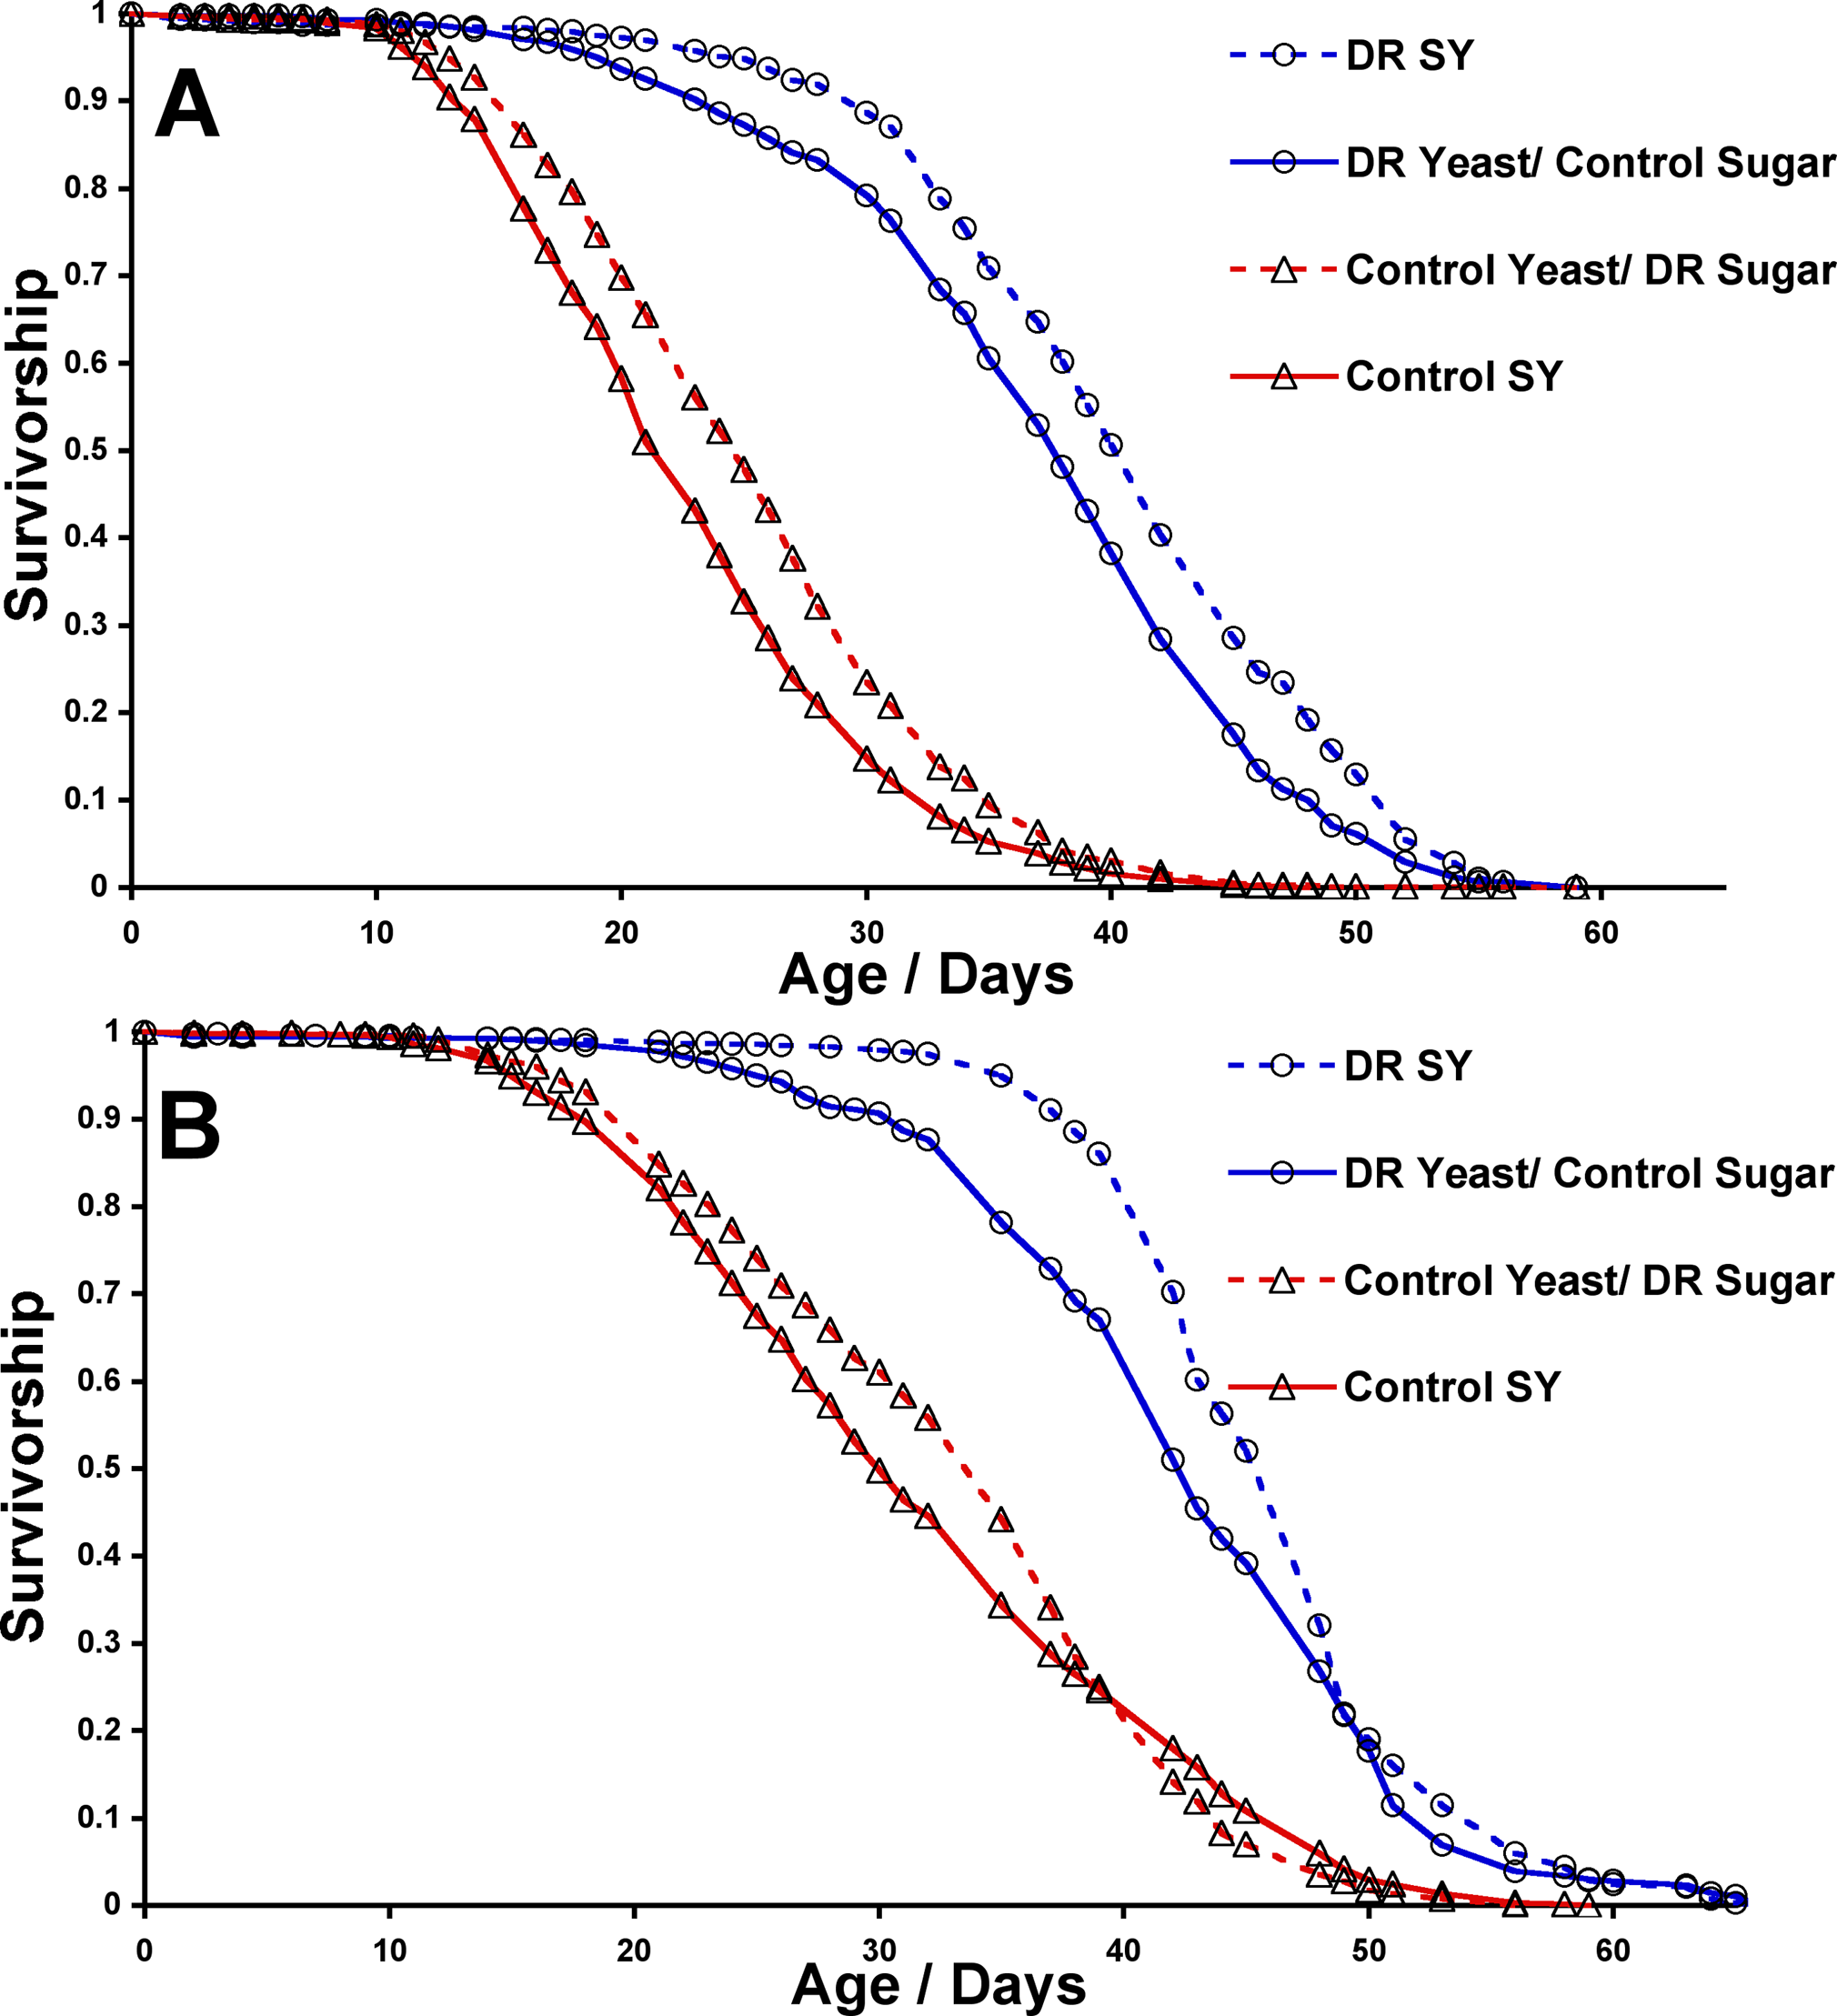
\includegraphics[height=0.85\textheight]{cr_lifespan_increase} \\
    Source: \cite{mair2005calories}
    \pnote{
        Originally caloric restriction \\
        Experiment showed: not just calories \\
        Has been replicated as well \\
        Lifespan increase 20-40\% \\
        A/B replication of same setup
        \par
        Visible: does not just depend on calories \\
        Also well-established in Humans
        \par
        Next: Why does this work? What does it do? \\
    }
\end{frame}

\begin{frame}[c]{Dietary Restriction Pathways in Yeast}
    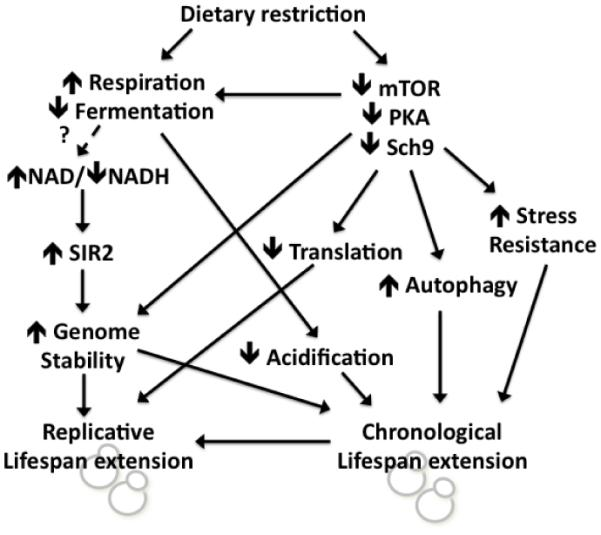
\includegraphics[height=0.85\textheight]{dietary_restrict_yeast} \\
    Source: \cite{kapahi2017dietary}
    \pnote{
        Fruit fly much more confusing, but similar
        \par
        Downregulation of mTOR receptors \\
        (mechanistic Target of Rapamycin)
        \par
        SIR -> increased dna damage repair \\
        Autophagy -> usually 10-20\% non-func protein \\
        'Starvation Mode': Be more efficient \\
        (also downregulate immune system)
        \par
        Next: Dietary Restriction Effects
    }
\end{frame}


\begin{frame}[c]{Dietary Restriction Effects}
    \large
    \begin{itemize}[<+(1)->]
        \item 'Different' mitochondrial energy production (less ROS)
        \item Reduced protein synthesis, no dna duplication
        \item Increased repair capacity (SIRT and others)
        \item Increased removal of misfolded proteins
        \item Reduced intracellular (oxidative) stress
        \item Reduced inflammation and proliferation
    \end{itemize}
    \pause
    Overall: Optimizing energy and resource usage
    \pnote{
        ROS = Reactive Oxygen Species, damage-inducing \\
        Usual mode: just blast through / press ahead \\
        "Ohne Rücksicht auf Verluste" \\
        Less safety checks and enthusiastic production
        \par
        Works, as usually enough energy is present \\
        Also: Mitochondrial downregulation \\
        Proliferation: cell division and protein synthesis
        \par
        Maybe we can target these pathways directly? \\
        Next: Inhibiting mTOR receptors
    }
\end{frame}


\begin{frame}[c]{Inhibiting mTOR receptors}
    \large
    Nutrient-Sensing pathways:
    \begin{itemize}[<+(1)->]
        \item AMPK
        \item mTOR
        \item IGF-1
    \end{itemize}

    \pause
    Medications \textbf{in trial} to affect these pathways:
    \begin{itemize}[<+(1)->]
        \item Metformin \cite{TAMETarg47:online}
        % \item Metformin \cite{martin2013metformin}, \cite{TAMETarg47:online}
        \item Rapamycin \cite{Particip66:online}
        \item Many more ...
    \end{itemize}
    \pnote{
        AMPK = 5' AMP-activated protein kinase \\
        AMP = Adenosine Monophosphate = ATP -2P \\
        IGF-1 = Insulin-like-Growth-Factor 1 \\
        \par
        Large-scale studies to achieve same benefits \\
        without actual dietary restriction \\
        \par
        So how does it fare? How do they do? \\
        Next: Evaluation
    }
\end{frame}


% \begin{frame}[c]{mTOR Inhibitors (Metabolic manipulation)}
%     Dietary restriction has been shown to extend healthy lifespan across several species. Drugs that mimic the metabolic effects of dietary restriction also have beneficial effects on lifespan. Nutrient-sensing biochemical pathways (such as IGF-1, mTOR and AMPK) play a key role in these effects. Metformin is a drug that is FDA-approved for diabetes that extends healthy lifespan in mice by inhibiting mTOR and activating autophagy. Metformin is currently being tested in a large clinical trial in humans to test its anti-aging properties.

% Source: here
% Hallmarks of aging targeted: The widespread mechanisms of action of metformin help to improve all of the 9 hallmarks of aging, shown below. I'll save the details for those interested, who can read a more thorough review here.

% Source: here.
% Another promising drug that manipulates metabolism is rapamycin (also known as siromilus), an FDA-approved immunosuppressant that extends healthy lifespan in mice and similarly acts to inhibit mTOR. Rapamycin is currently in a clinical trial in humans to test its anti-aging properties.
% \end{frame}


\begin{frame}[c]{Method Evaluation: Metabolic Manipulation}
    \textbf{Hallmarks affected}: \\
    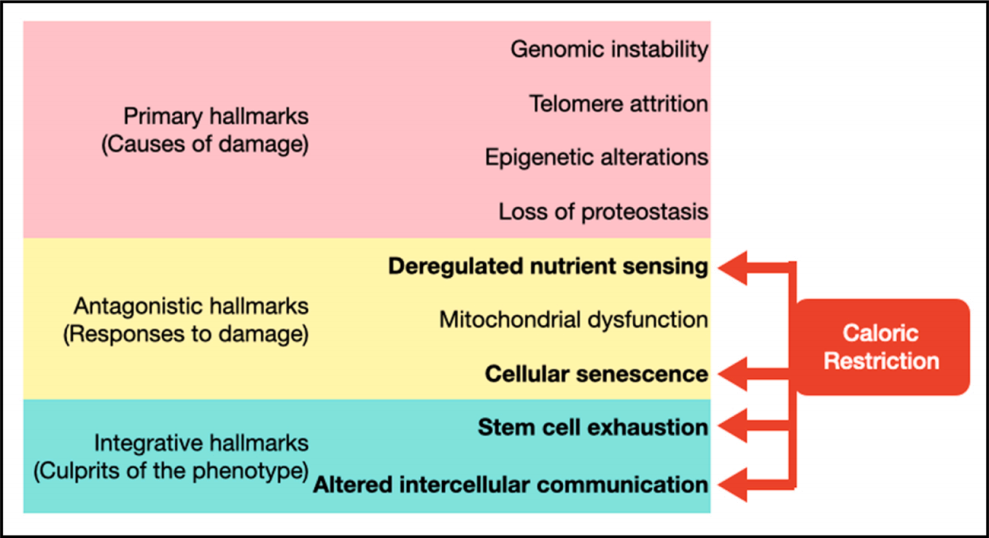
\includegraphics[width=0.8\textwidth]{cr_pathway_effects} \\
    Source: \cite{erbaba2020effects} \\
    \pause
    Lifespan extension: about 20-40\% QUALY \cite{swindell2012dietary} \\
    \pause
    \textbf{State: In clinical trial}, e.g. \cite{TAMETarg47:online}
    \pnote{
        More of a 'slow down', preventing worst case \\
        Not silver bullet, rather 'one-trick pony' \\
        Not clear that this is correct classification
        \par
        Not 'root-cause' prevention \\
        but still amazing progress \\
        \par
        Next: Senolytics
    }
\end{frame}


\subsection{Senolytics}

\begin{frame}[c]{Senescent Cells: What are they?}
    \large
    \begin{itemize}[<+(1)->]
        \item Old or (partially) damaged cells
        \item Sending out Senescence-Associated Secretory Phenotype (SASP)
        \item SASP causes inflammation and age-related diseases, e.g. Arthritis, Atherosclerosis
        \item Cells induce apoptosis (suicide) or wait to get removed by immune system
        \item About 8\% of cells in young, and 17\% of cells in old mice are senescent \cite{folgueras2018mouse}
    \end{itemize}
    \pnote{
        SASP part of damage-fallback state \\
        'I won't be able to fix this' \\
        Zombie-like death-resistent cells
        \par
        Very interesting: senescent difference \\
        in old vs young mice \\
        \par
        Next: Deeper look at SASP effects
    }
\end{frame}

\begin{frame}[c]{Senescent Cell Effects}
    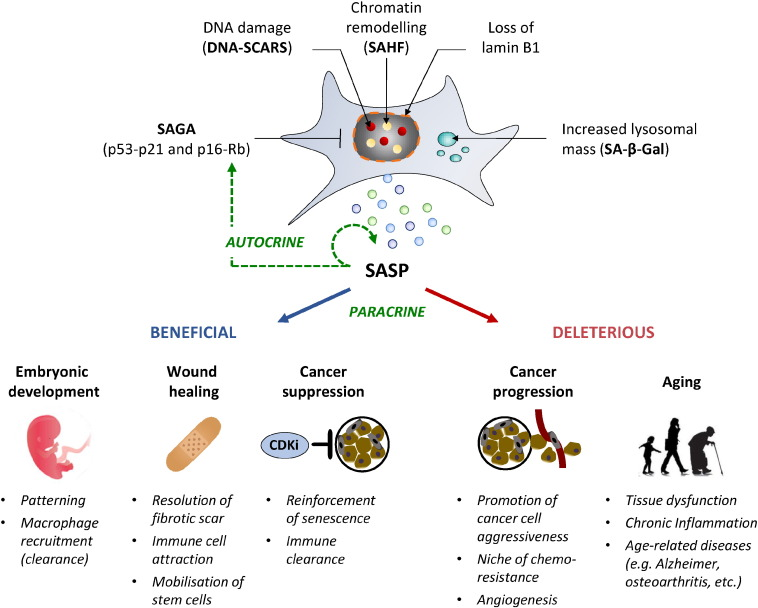
\includegraphics[height=0.85\textheight]{sasp_effects} \\
    Source: \cite{malaquin2016keeping}
    \pnote{
        SASP meant to increase cell-turnover \\
        more apoptosis, more cell growth to replace \\
        less 'safety checks' with high proliferation
        \par
        also toxic agents + ROS to make less hospitable \\
        specific factors induce cell death and growth
        \par
        good for wound healing (high turnover) \\
        Klassisch: 'Entzündung' (inflammation)
        \par
        Next: Senolytic Uses and Effects
    }
\end{frame}


% \begin{frame}<handout>[c]{Inflammation Effects}
%     \begin{aquote}{\cite{NintilTh68:online}}
%         {\em Also, the environment that inflammation creates is one that is} meant to
%         increase cell turnover {\em (More apoptosis, but also more cell growth to
%         replace lost cells), with granulocytes secreting toxic agents
%         (Including ROS) to make the area affected less hospitable (But also
%         increases damage to DNA), and specific cytokines like the} tumor
%         necrosis factor that induce cell death, and growth factors that promote
%         cell growth.
%     \end{aquote}
% \end{frame}

\begin{frame}[c]{Senolytics: Uses and Effects} 
    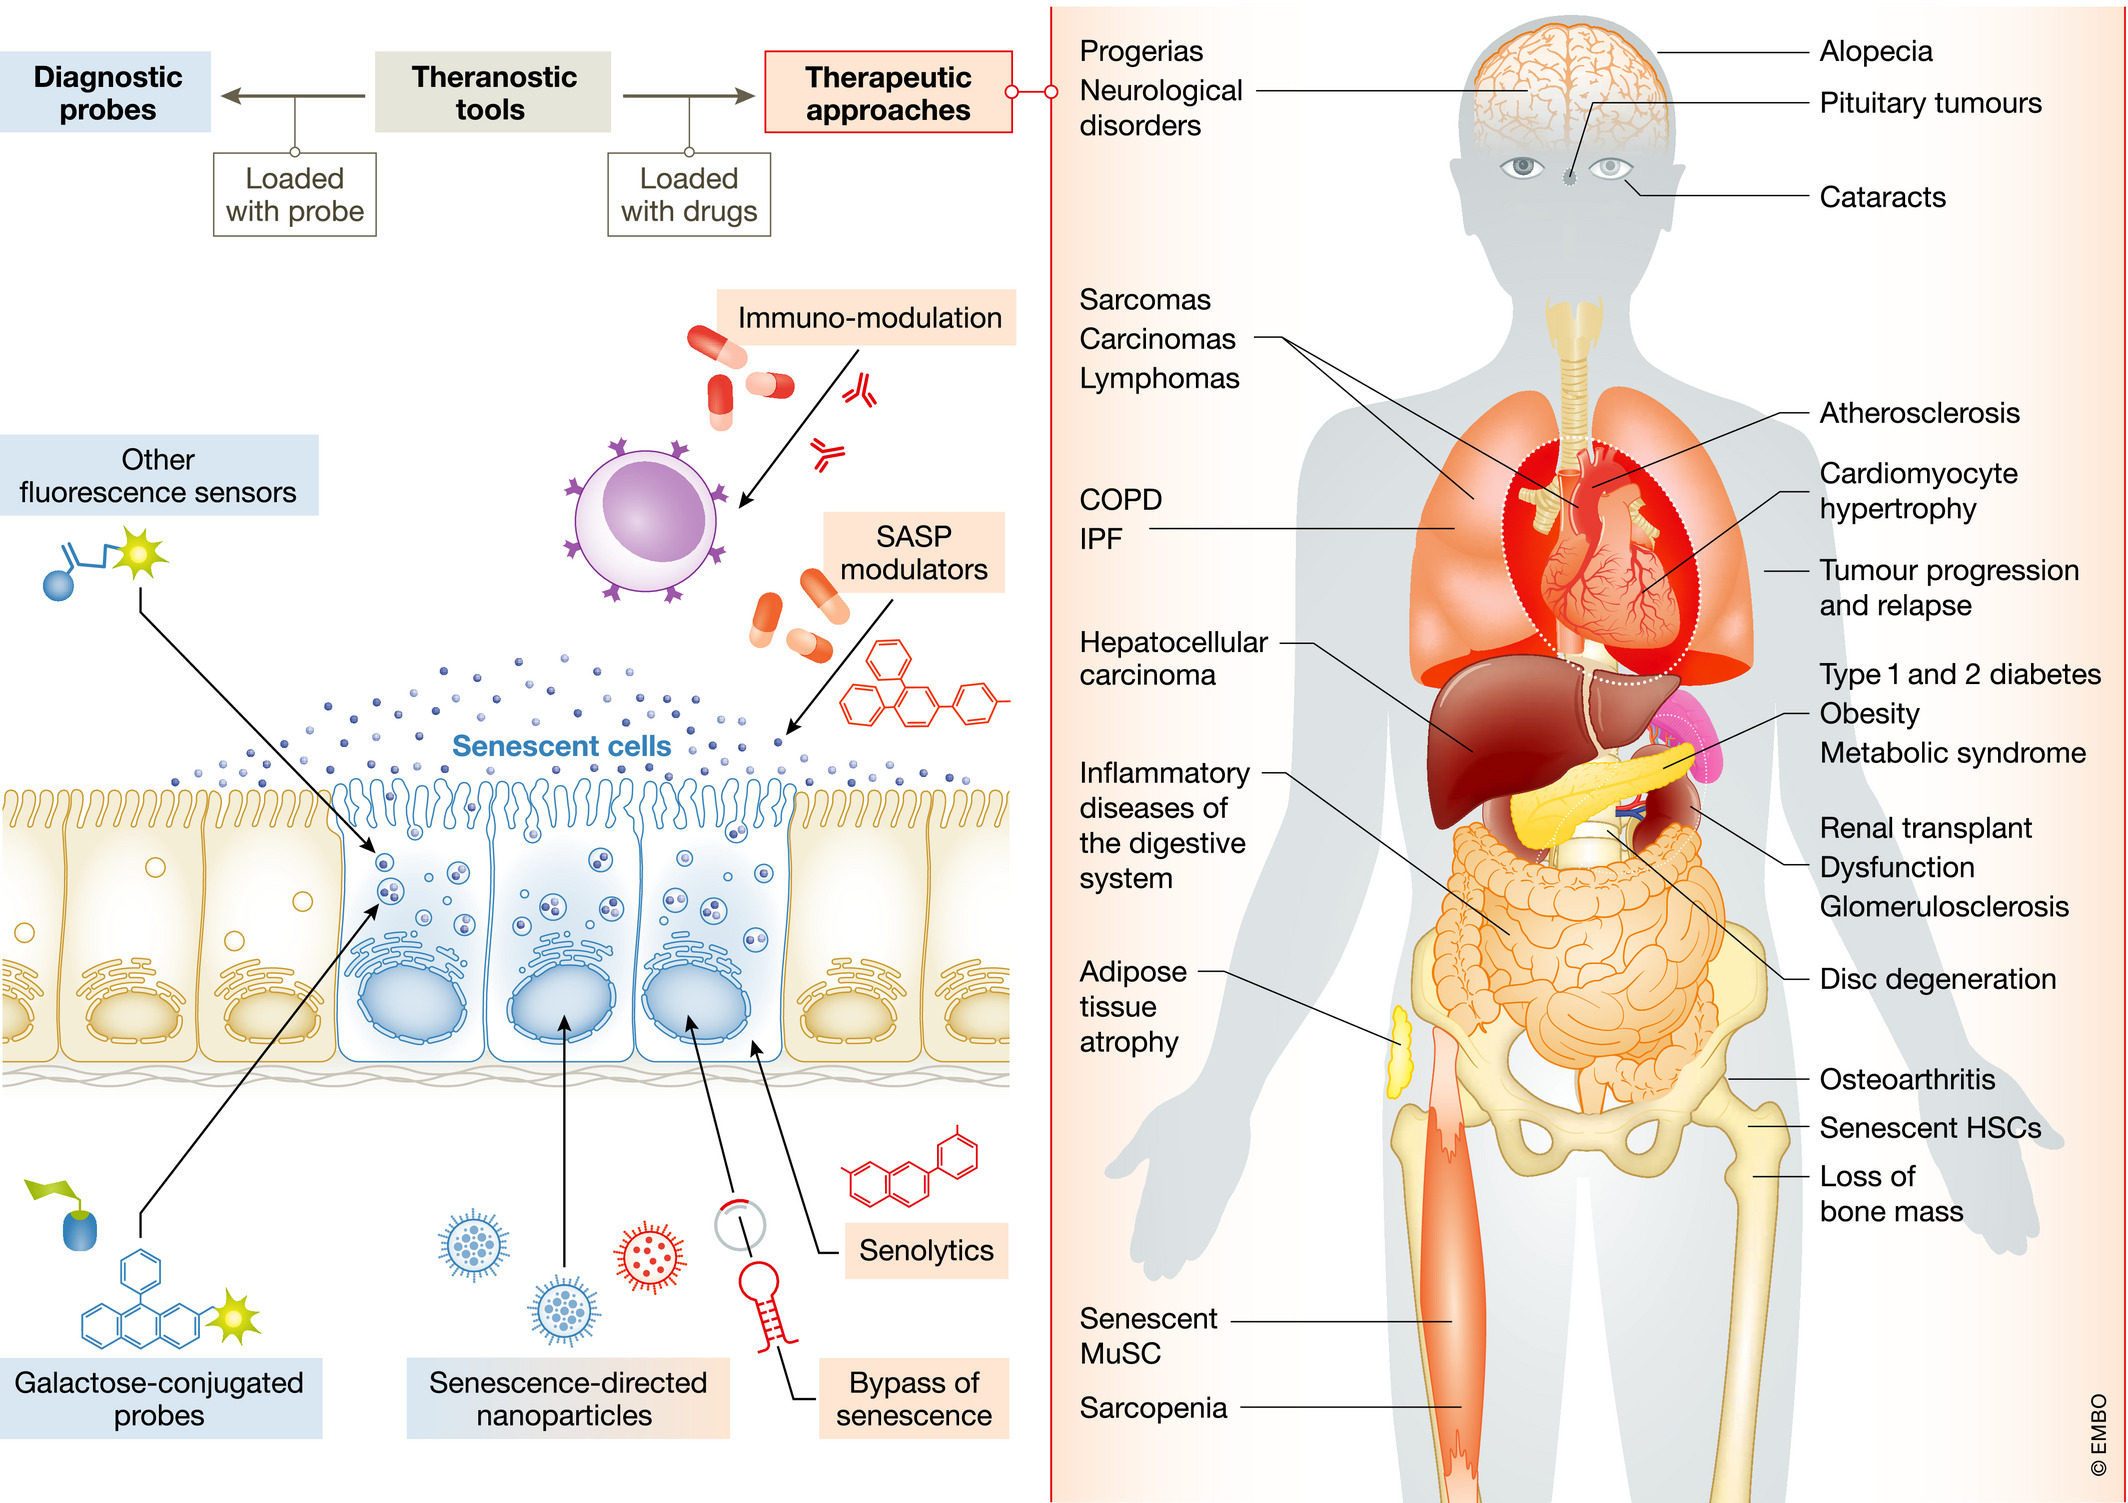
\includegraphics[height=0.85\textheight]{senescent_strategies} \\
    Source: \cite{paez2019targeting}
    \pnote{
        Right: Inflammation Diseases, usually when old \\
        Left: \\
        - e.g. Probes to detect senescence \\
        - Senolytics: inhibit pro-survival pathways \\
        -   Increasing apoptosis and immuno-clearance \\
        - SASP modulation: inhibit negative effects \\
        - Immuno-": Promote immune system clearance
        \par
        Next: Evaluation
    }
\end{frame}

% \begin{frame}[c]{Senolytics (Drugs killing senescent cells)}
%     Senescent cells are a kind of 'zombie'-like cell that accumulate with age. They are death-resistant cells that secrete proinflammatory factors associated with a range of age-related diseases (below, right):

% Cellular senescence is associated with multiple human disorders. The development of galactose‐conjugated and fluorescent probes to detect and highlight senescent cells offers an important opportunity for longitudinal monitoring of senescence in clinical trials. Pharmacologically active small compounds known as senolytics inhibit pro‐survival pathways in senescent cells leading to apoptosis, a therapeutic strategy that may additionally be enhanced by the use of immune modulators promoting natural clearance of senescent cells. Finally, nanoparticles encapsulating cytotoxic drugs, tracers and/or small molecules can be used as theranostic tools, both for therapeutic and diagnostic purposes. Source: here
% There are various strategies being explored to kill or reprogram senescent cells (above, left), including senolytics. Senolytics are drugs that kill senescent cells to improve physical function and healthy lifespan. When administered to older mice, senolytics have been shown to reverse many aspects of aging such as cataracts, and arthritis (below):

% Killing senescent cells with senolytics extends the median healthy lifespan by up to 27\% in mice (below). Several senolytics, such as the combination of dasatinib and quercetin, and fisetin are in clinical trials in humans today.

% Study design for clearance of senescent cells mouse cohort. Median survival (in days, d) and percentage increase in median survival are indicated. Source: here
% Hallmarks of aging reversed: senolytics decelerate cellular senescence, improve epigenetic markers and restore intercellular communication (by reducing inflammation associated with senescent cells) to extend healthy lifespan.
% \end{frame}


\begin{frame}[c]{Method Evaluation: Senolytics}
    \textbf{Hallmarks affected}: \\
    \begin{itemize}[<+(1)->]
        \item Decelerate Cellular Senescence
        \item Improve Epigenetic Markers
        \item Restore Intercellular Communication (by reducing inflammation associated with senescent cells)
    \end{itemize}
    \pause
    Lifespan extension: 27\% median Life\\
    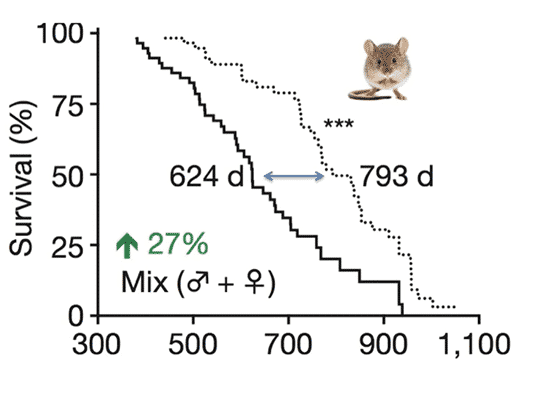
\includegraphics[width=0.4\textwidth]{senolytics_extend_life}
    Source: \cite{baker2016naturally} \\
    \pause
    \textbf{State: In clinical trial}
    \pnote{
        Going much more in on root causes \\
        Depends heavily on immune system capacity \\
        \par
        Bonus: Very different mechanism, \\
        so probably good complement to other methods \\
        \par
        Next: Cellular Reprogramming
    }
\end{frame}


\subsection{Cellular Reprogramming}

\begin{frame}[c]{(Epigenetic) Cellular Reprogramming: What is it?} 
    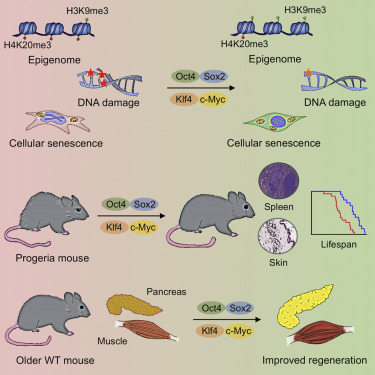
\includegraphics[height=0.85\textheight]{repr_overview} \\
    Source: \cite{ocampo2016vivo}
    \pnote{
        The idea is to 'reprogram' old cells \\
        to be like young cells
        \par
        Largely dependent on epigenome: dna markers \\
        Goal: Basically to reprogram the epigenome
        \par
        Next: Epigenetics
    }
\end{frame}


\begin{frame}[c]{Epigenetics: What is it?}
    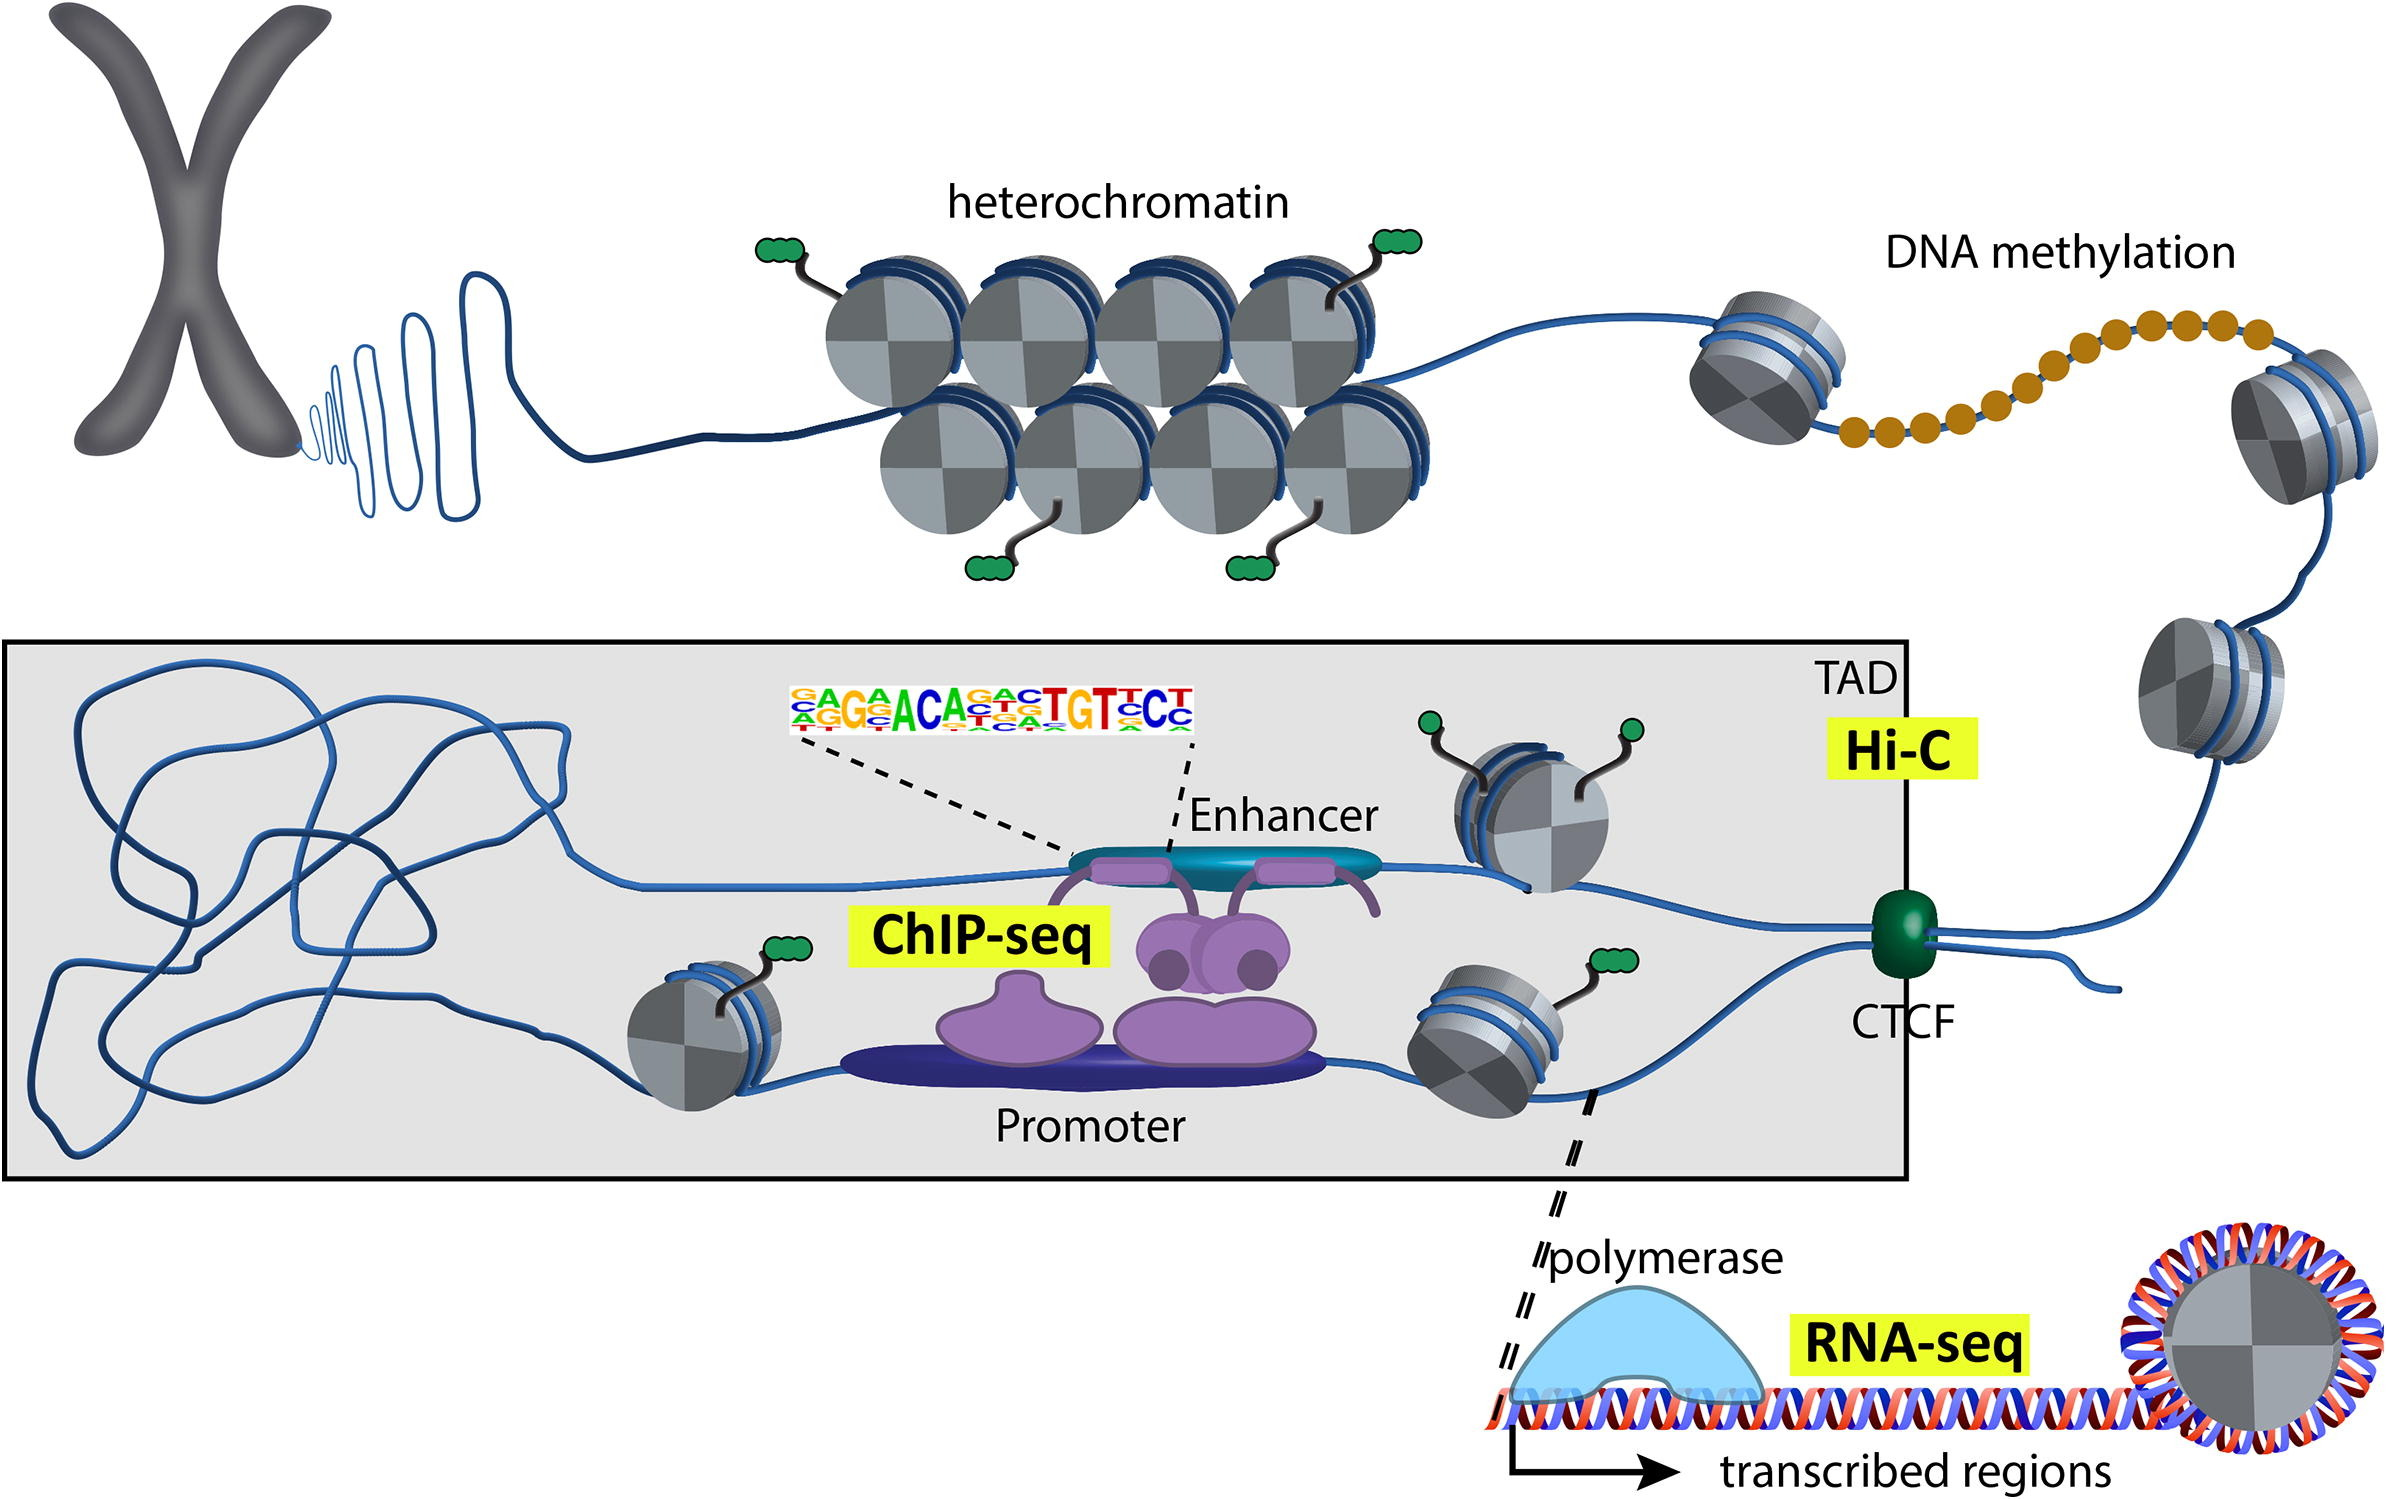
\includegraphics[height=0.85\textheight]{epigenetics} \\
    Source: \cite{hollbacher2020seq}
    \pnote{
        Epigenetics: many state machines as to \\
        what the cell is supposed to be doing \\
        by methylation certain parts of the genome \\
        can be modulated by messages/hormones
        \par
        decides which genes are being expressed/suppressed \\
        Can be thought of as 'cell identity' \\
        differentiation between muscle cell and skin cell
        \par
        'highest-level' regulation of what happens \\
        Danger lies in 'forgetting' own states \\
        Next: Cellular Reprogramming
    }
\end{frame}

\begin{frame}[c]{(Epigenetic) Cellular Reprogramming: What is it?}
    \large
    \begin{itemize}[<+(1)->]
        \item Basically: reset the corroding Epigenetic state to a 'younger' and functional one
        \item In fact, we can create induced pluripotent stem cells (iPSC) \cite{takahashi2006induction}
        \item Cells activated with Yamanaka-factors are indistinguishable (regarding aging-hallmarks) from younger versions of themselves
        \item Idea: only activate them long enough to reverse aging hallmarks, but keep cell identity
        \item Seems to complement well with senolytics \cite{ofenbauer2019strategies}
    \end{itemize}
    \pnote{
        When things start to go wrong, \\
        reset to a 'known working state'
        \par
        Originally, iPSC lost their cell identity \\
        iPSC more powerful and rare than stem cells
        \par
        Incredible potential for other treatments
        \par
        Next: Evaluation
    }
\end{frame}

% \begin{frame}[c]{Cellular Reprogramming}
%     Cellular reprogramming is the conversion of terminally differentiated cells (old cells) into induced pluripotent stem cells (IPSCs) (‘young’ cells). Cells can be re-programmed to a youthful state using a cocktail of 4 factors known as Yamanaka factors, a finding for which a Nobel prize was awarded in 2012.

% Induced pluripotent stem cells (IPSCs) have essentially unlimited regenerative capacity and carry the promise for tissue replacement to counter age-related decline. Partial reprogramming in mice has shown promising results in alleviating age-related symptoms without increasing the risk of cancer.

% (A) The diagram depicts cellular programming to pluripotency, in other words, the conversion of terminally differentiated somatic cells into induced pluripotent stem cells (iPSCs) by cellular reprogramming through forced expression of Yamanaka factors (Oct4, Sox2, Klf4, and c-Myc). (B) The diagram depicts the rejuvenation of aged cells by cellular reprogramming. The process results in the amelioration of hallmarks of aging such as mitochondrial dysfunction, shortening of telomere length, changes in epigenetic marks, increased DNA damage, and senescence. Source: here.
% An impressive example of cellular reprogramming was the restoration of vision in blind mice with a severed optic nerve using 3 of the 4 Yamanaka factors. The researchers from Harvard Medical School were able to regrow a fully functioning optic nerve in mice using cellular reprogramming. This approach could be used in future to regenerate other tissues as a new anti-aging strategy.

% Using the eye as a model tissue, expression of Oct4, Sox2 and Klf4 genes (OSK) in mice resets youthful gene expression patterns and the DNA methylation age of retinal ganglion cells, promotes axon regeneration after optic nerve crush injury, and restores vision in a mouse model of glaucoma and in normal old mice. Source: here.
% Hallmarks of aging targeted: Cellular reprogramming has been shown to reverse many of the hallmarks of aging, such as mitochondrial dysfunction, shortening of telomere length, changes in epigenetic marks, genomic instability, and cellular senescence.
% \end{frame}


\begin{frame}[c]{Method Evaluation: Cellular Reprogramming}
    \large
    \textbf{Hallmarks affected}: \\
    \begin{itemize}[<+(1)->]
        \item Mitochondrial Dysfunction
        \item Shortening of Telomere length
        \item Changes in Epigenetic markers
        \item Genomic Instability
        \item Cellular Senescence
    \end{itemize}
    \pause
    Lifespan extension: maximum by 20\% and median by 33\% \cite{ocampo2016vivo} \\
    \pause
    \textbf{State: in clinical trial}
    \pnote{
        mitochondrial function regulated by epigenetics \\
        energy-fail-states exist and hard to get out of \\
        stem cells have active telomerase \\
        close-to-senescent stem cells might exist, ask
        \par
        Next: Other Approaches
    }
\end{frame}



\subsection{Other Approaches}

\begin{frame}[c]{Other Promising Approaches}
    \large
    \begin{itemize}[<+(1)->]
        \item Thymic rejuvenation has been shown to reverse biological age in humans \cite{fahy2019reversal}
        \item Sirtuin enzyme activation \cite{mohar2012sirtuin}
        \item Boosting mitochondrial function with NAD+ precursor molecules \cite{aman2018therapeutic}
        \item Identifying genetic Markers \cite{kenyon2010genetics}
        \item Many more ...
    \end{itemize}
    \pnote{
        SIRT are part of DNA damage repair pathways \\
        NAD is being consumed in emergency response \\
        NAD = Nicotinamide adenine dinucleotide \\
        Preventing dangerous mitochondrial fail-states \\
        Unclear how genetic markers affect longevity
        \par
        Next: Evaluation
    }
\end{frame}


\begin{frame}[c]{Method Evaluation: Other Approaches}
    \large
    \textbf{Hallmarks affected}: ??? \\
    \pause
    Lifespan extension: Most 5\%-40\% \\
    \pause
    State: Active research, some in animal or clinical trials
    \pnote{
        A lot of different approaches \\
        Many with as-yet-unknown effects on vertebrates \\
        yet others already in clinical trials \\
        All of what I'm presenting is active research
        \par
        Ask me about state of yeast
        \par
        Next: What can I do?
    }
\end{frame}
